\section{Rozbudowa obudowy robota}
Obudowa robota Dark Explorer stworzona w ramach poprzedniej pracy magisterskiej
\cite{KmakMScThesis2009} składała się z dwóch elementów bazowych. Pierwszym
elementem jest podwozie wykonane ze spienionego PCW o grubości 6mm. Głównym jego
zadaniem jest zapewnienie ochrony wszystkim podzespołom elektronicznym
zainstalowanym w robocie, jak również dostarczenie punktów mocowania
pozwalających na integrację poszczególnych grup funkcjonalnych. Drugim ważnym
elementem jest pokrywa wierzchnia wykonana z przeźeoczystej płyty pleksi na
której zamonotowany został serwomechanizm z wieżą na której zamontowana została
kamera. Całość po zmontowaniu prezentuje się w sposób pokazany na rysunku
\ref{fig:DESideView}.

\begin{figure}[h!]
 \centering
 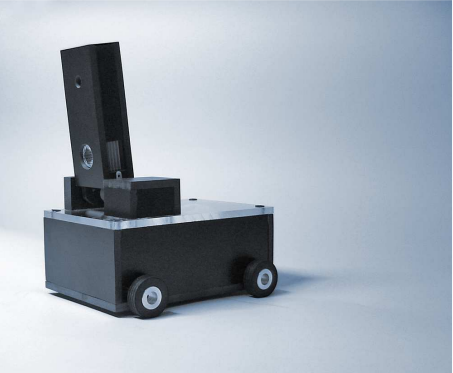
\includegraphics[height=100mm]{../images/ch04/de_side_view.png}
 \caption{Wygląd robota po zmontowaniu wszystkich elementów}
 \label{fig:DESideView}
\end{figure}

Ze względu na dużą ilość czujników dodatkowych których obsługa została dodana w
obecnej wersji robota, wszelkie próby wykorzystania istniejącej obudowy
zakończyły się niepowodzeniem. Dlatego też zaprojektowany został ekspander
pozwalający w ławty sposób zintegrować poprzednią konstrukcję z zestawem nowych
czujników i urządzeń peryferyjnych. Wspomniany ekspander ma postać
prostopadłościanu wykonanego w całości z płyt bezbarwnej pleksi. 
Wszystkie elementy elektroniczne zostały rozmieszczone na spodniej płycie
ekspandera, a potrzebne połączenia zostały wyprowadzone poprzez otwory z
gniazdami zainstalowanymi w miejscu podłączenia czujnika. Schemat projektowy
dolnej płyty ekspandera widoczny jest na rysunku \ref{fig:SensorsBoard}.

\begin{figure}[h!]
 \centering
 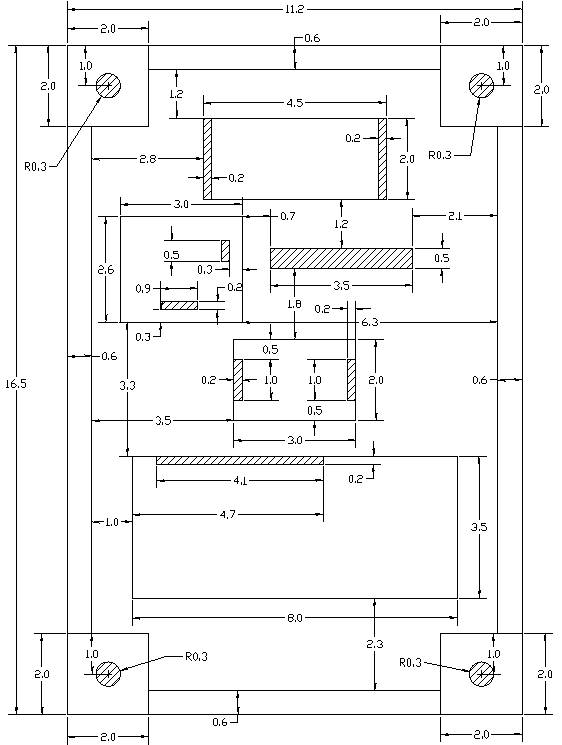
\includegraphics[height=150mm]{../images/ch04/sensor_board.png}
 \caption{Wygląd robota po zmontowaniu wszystkich elementów}
 \label{fig:SensorsBoard}
\end{figure}

W centrum ekspandera umiejscowiony został żyroskop, celem takiego zabiegu było
wyeliminowanie potencjalnych problemów związanych z pomiarem kąta o jaki robot
się obrócił w przypadku gdy czujnik pomiarowy nie znajduje się na osi wzdłuż
której obrót jest dokonywany. W południowej części umieszczony został
wyświetlacz LCD za pomocą którego użytownik będzie mógł na bierząco monitorować
aktualne działania robota. W północnej części zamontowany został akcelerometr
oraz magnetometr. Taka konfiguracja pozwoliła na ograniczenie ilości i długości
przewodów potrzebnych do podłączenia wszystich elementów do płyty głównej robota
